% Preámbulo
\documentclass[a4paper,11pt]{article}
% Paquetes
\usepackage[latin1]{inputenc}
\usepackage{color}
\usepackage{array}
\usepackage{amsmath,amssymb}
\usepackage{graphicx}

\addtolength{\textwidth}{2cm}
\addtolength{\hoffset}{-1cm}

\title{Donald E. Knuth: Datos bibliográficos}
\author{Perico de los Palotes}

% Entorno del documento
\begin{document}

\maketitle

\tableofcontents

\section{Introduction}
Donald E. Knuth (born January 10, 1938) is a computer scientist 
and Professor Emeritus of the Art of Computer Programming at 
Stanford University \cite{unistan}.

Author of the seminal multi-volume work The Art of Computer Programming \cite{acp}, 
Knuth has been called the ``father'' of the analysis of algorithms, 
contributing to the development of, and systematizing formal mathematical 
techniques for, the rigorous analysis of the computational complexity of 
algorithms, and in the process popularizing asymptotic notation.

\subsection{\TeX creator}

In addition to fundamental contributions in several branches of theoretical 
computer science, Knuth is the creator of the TeX computer typesetting 
system, the related METAFONT font definition language and rendering system, 
and the Computer Modern family of typefaces.

A writer and scholar \cite{joke}, Knuth created the WEB/CWEB computer programming 
systems designed to encourage and facilitate literate programming, 
and designed the MMIX instruction set architecture.

\begin{figure}[h]
\begin{center} 
\bigskip
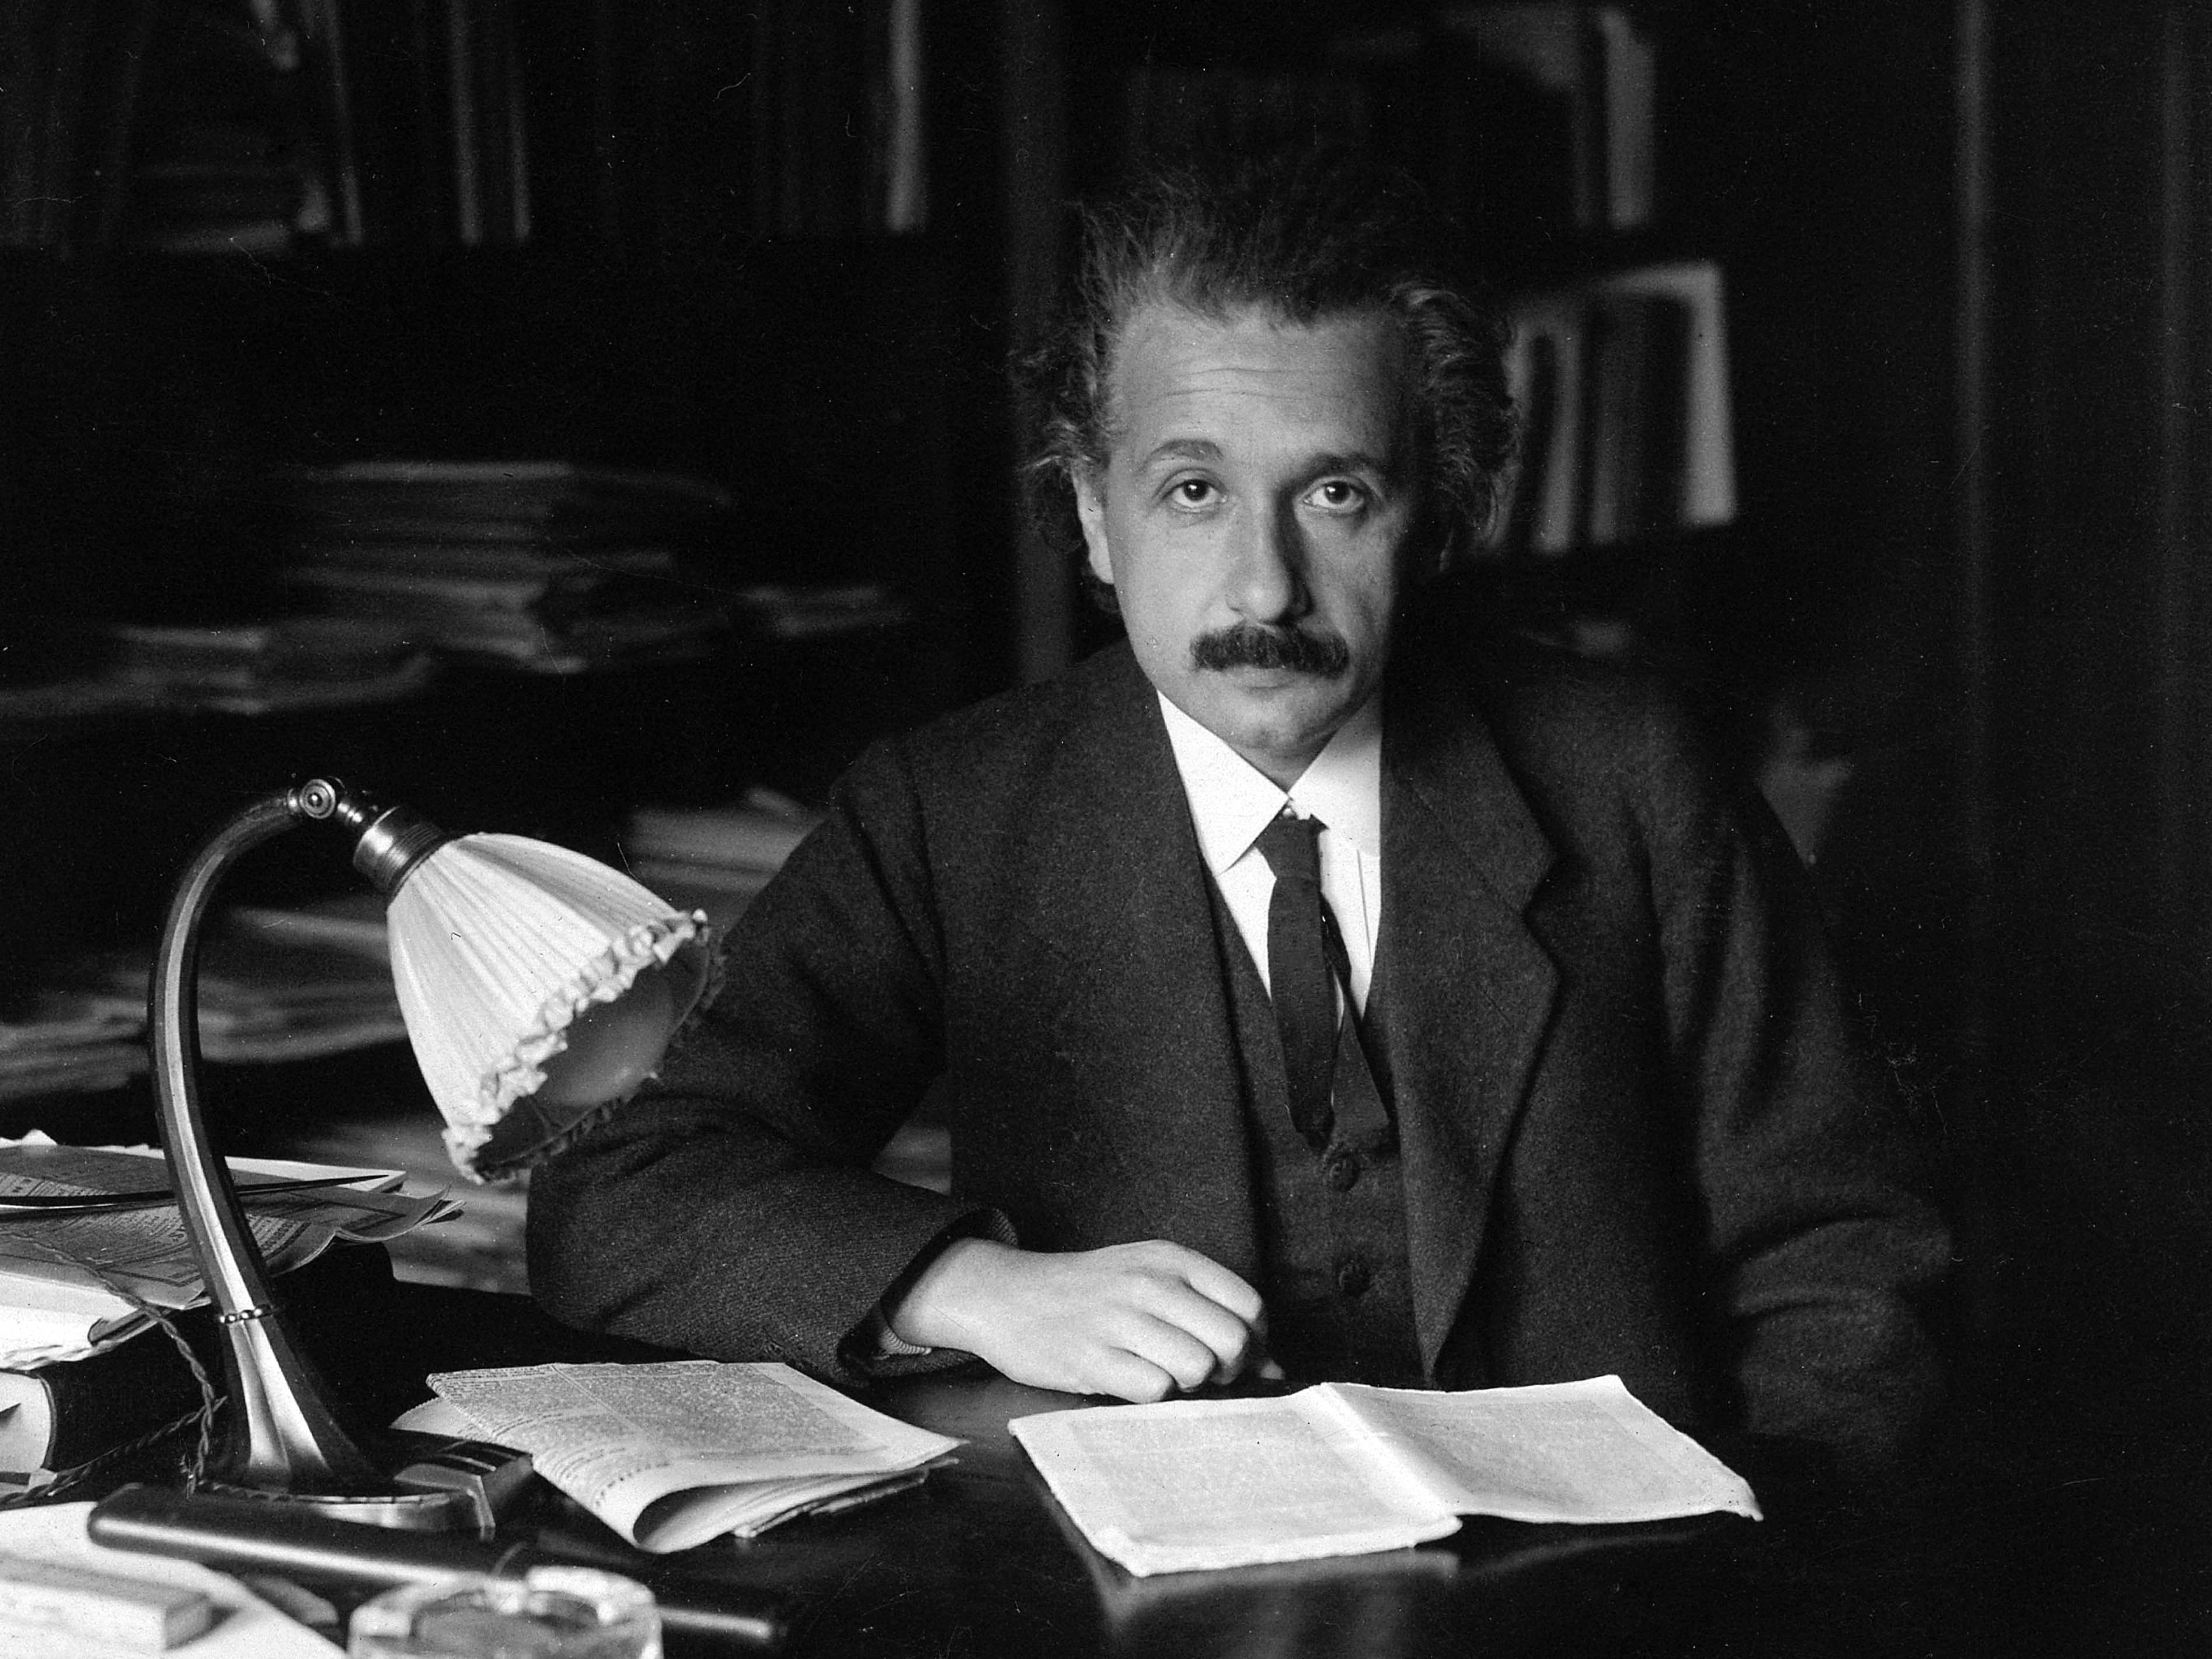
\includegraphics[trim=15 30 30 0,clip,height=0.3\textwidth]{Images/einstein.jpg} \hspace{5mm}
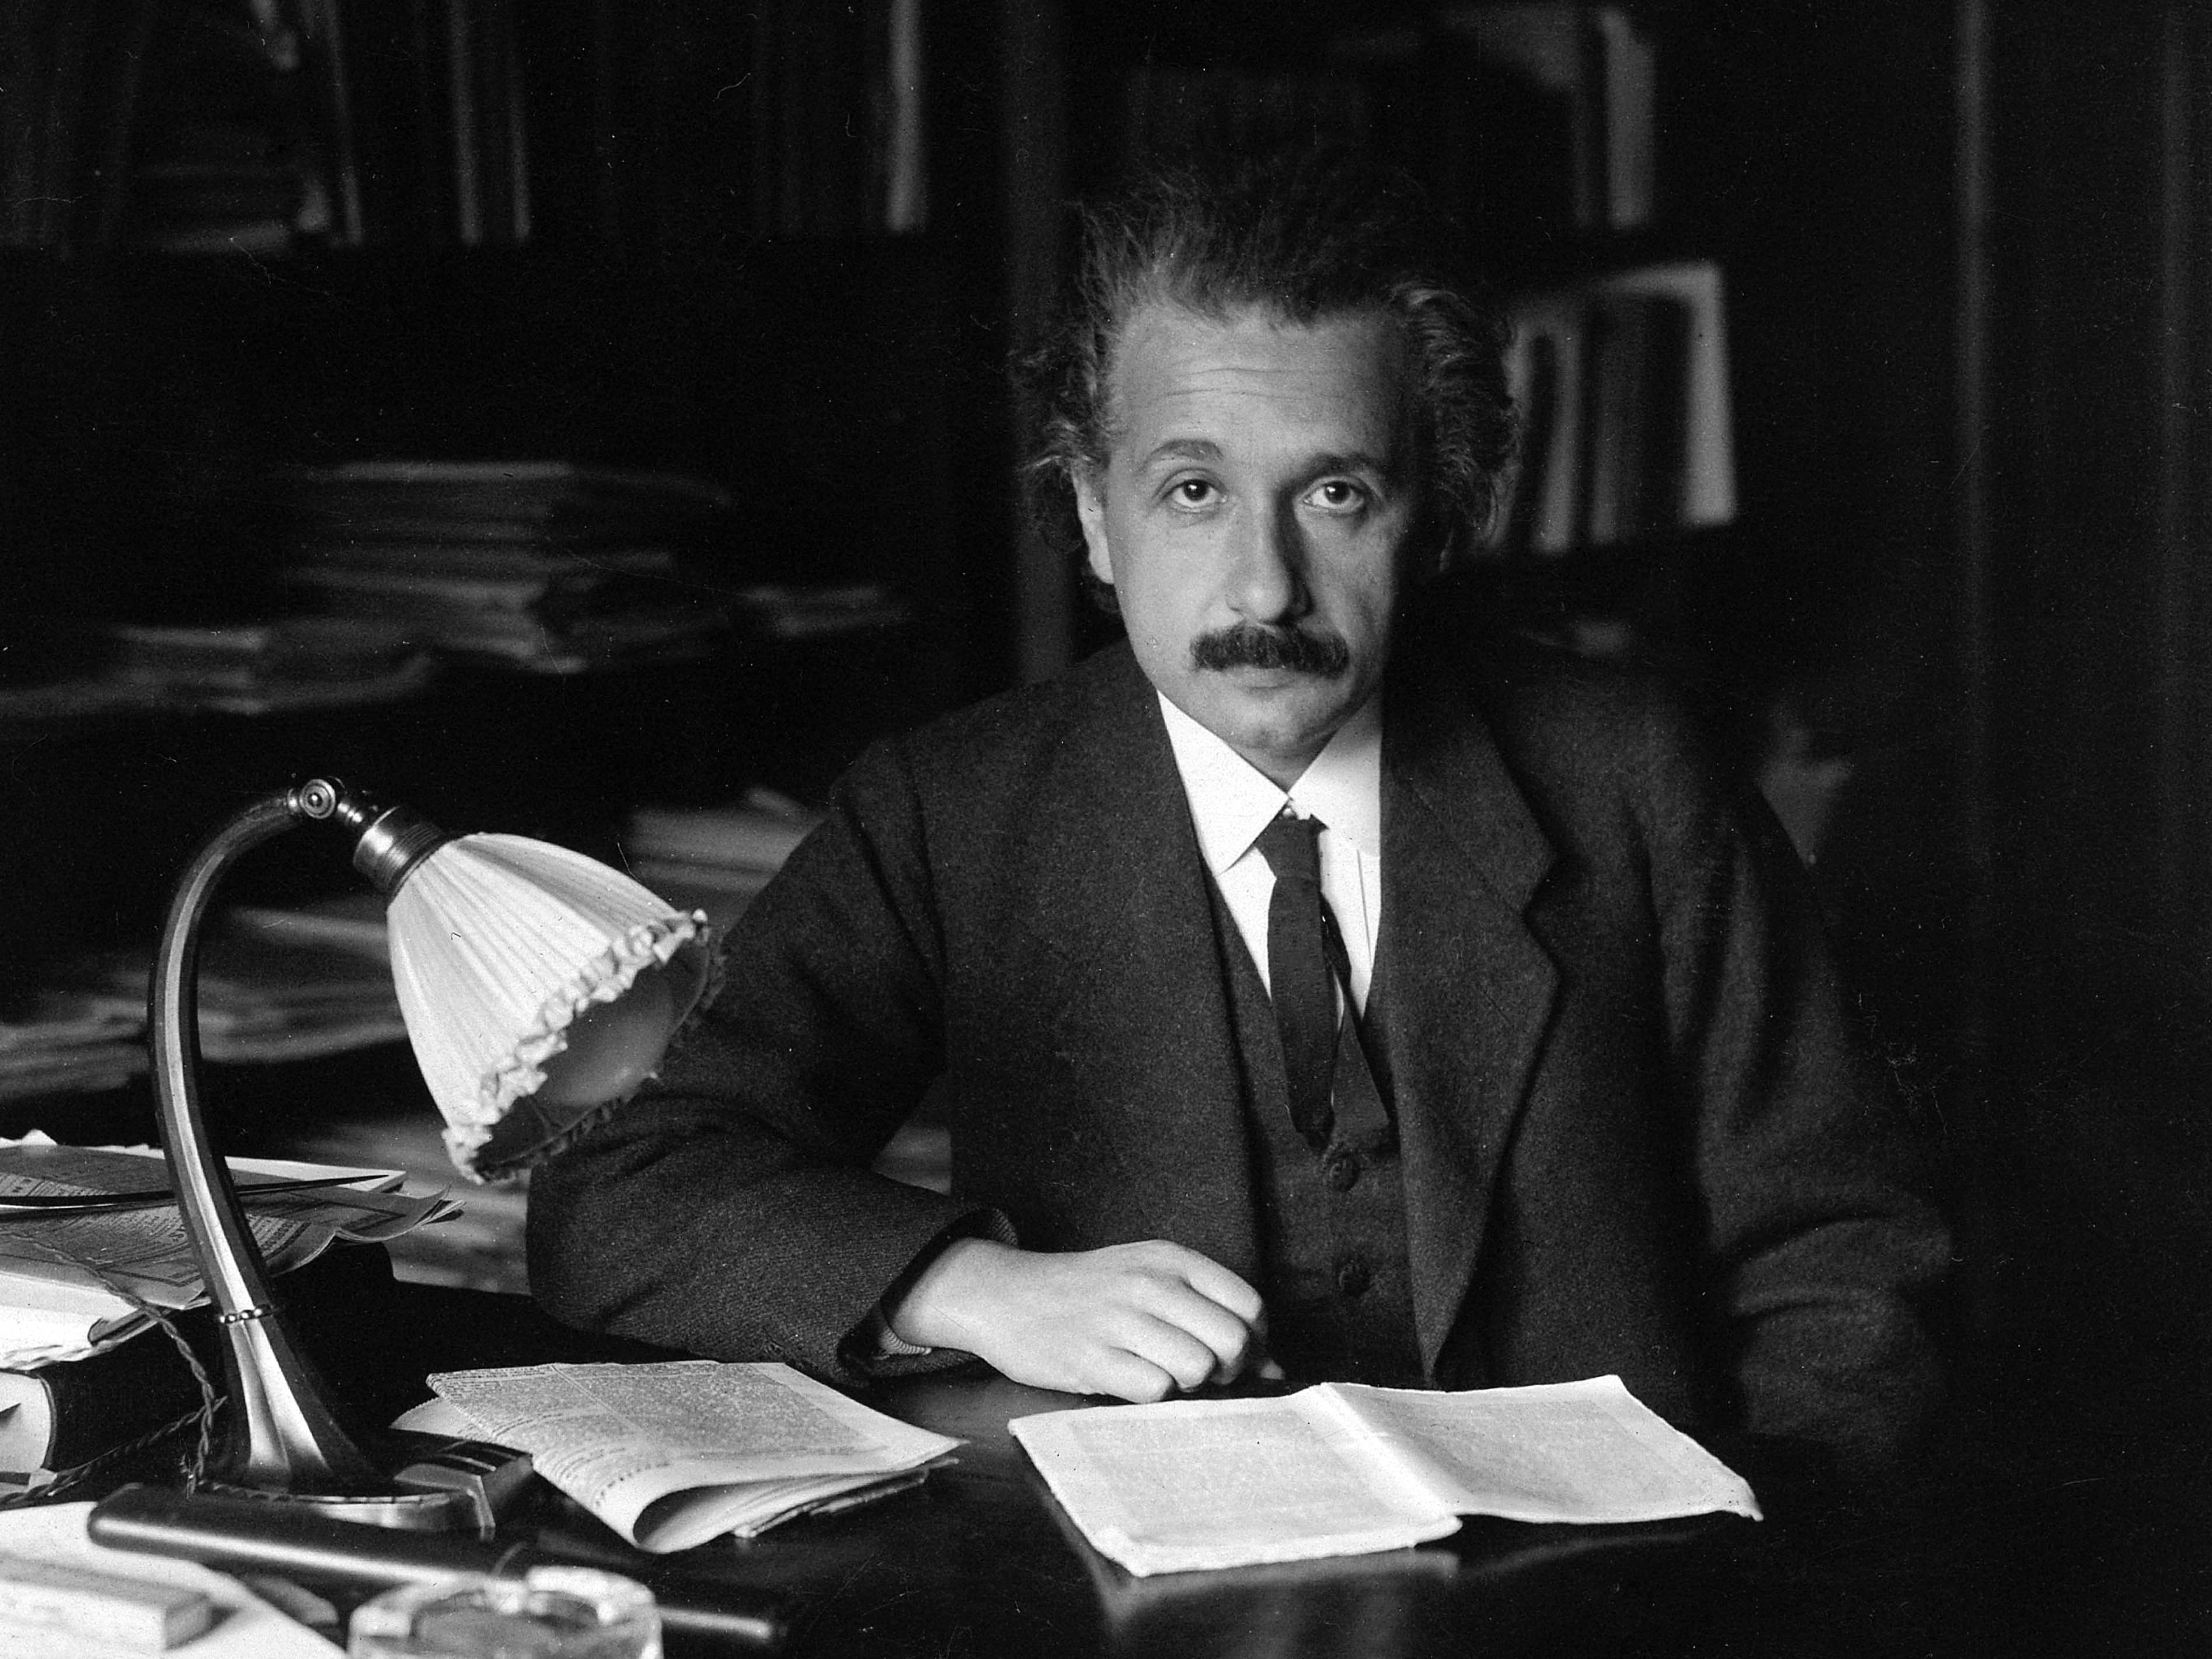
\includegraphics[origin=c,angle=180,height=0.3\textwidth]{Images/einstein.jpg}
\end{center}
\vspace{-5mm}
\caption{Donald E. Knuth, el creador del sistema TeX/LaTeX}
\end{figure}

\section{Education} 

\subsection{Childhood}
Knuth was born in Milwaukee, Wisconsin, where his father owned a small 
printing business and taught bookkeeping at Milwaukee Lutheran High 
School, which he attended. He was an excellent student, earning achievement 
awards. He applied his intelligence in unconventional ways, winning a contest 
when he was in eighth grade by finding over 4,500 words that could be formed 
from the letters in "Ziegler's Giant Bar." The judges had only about 
2,500 words on their master list. This won him a television set for his school 
and a candy bar for everyone in his class \cite{concurso}.

\subsection{College}
Knuth had a difficult time choosing physics over music as his major at Case 
Institute of Technology (now part of Case Western Reserve University). He 
also joined Theta Chi Fraternity. He then switched from physics to mathematics, 
and in 1960 he received his bachelor of science degree, simultaneously 
receiving his master of science degree by a special award of the faculty 
who considered his work outstanding. At Case, he managed the basketball 
team and applied his talents by constructing a formula for the value of 
each player. This novel approach was covered by Newsweek and by Walter 
Cronkite on the CBS television network. As an undergraduate at Case, 
Knuth was hired to write compilers for different computers.

\section{Academic work}

In 1963, he earned a Ph.D. in mathematics (advisor: Marshall Hall) from 
the California Institute of Technology, where he became a professor and 
began work on The Art of Computer Programming, originally planned to be 
a single book, and then planned as a six, and then seven-volume series. 
In 1968, he published the first volume. That same year, he joined the 
faculty of Stanford University, having turned down a job offer from 
the National Security Agency (NSA).

\begin{figure}[t]
\begin{center} 
\bigskip

\includegraphics[height=0.25\textwidth]{Images/linux-logo.jpg} \hspace{5mm}
\begin{tabular}[b]{|c|c|c|}
\hline
A & B & C  \\ \hline
Uno & Dos & Tres \\
Cuatro & Cinco & Seis \\ \hline
\end{tabular}
\end{center}
\vspace{-5mm}
\caption{El pingüino Tux y una tabla}
\label{tux}
\end{figure}

\section{Awards}
In 1971, Knuth was the recipient of the first ACM Grace Murray Hopper 
Award. He has received various other awards including the Turing Award, 
the National Medal of Science, the John von Neumann Medal, and the Kyoto 
Prize. After producing the third volume of his series in 1976, he 
expressed such frustration with the nascent state of the then newly 
developed electronic publishing tools (especially those that provided 
input to phototypesetters) that he took time out to work on typesetting 
and created the TeX and METAFONT tools.

In recognition of Knuth's contributions to the field of computer science, 
in 1990 he was awarded the one-of-a-kind academic title of Professor of 
The Art of Computer Programming, which has since been revised to Professor 
Emeritus of The Art of Computer Programming.

\textbf{Aquí citamos (mediante referencias cruzadas) la figura \ref{tux}}

\section{Memberships}
In 1992 he became an associate of the French Academy of Sciences. Also
 that year, he retired from regular research and teaching at Stanford 
University in order to finish The Art of Computer Programming. In 2003 
he was elected as a foreign member of the Royal Society. As of 2004, 
the first three volumes of his series have been re-issued, and Knuth is 
currently working on volume four, excerpts of which are released periodically 
on his website. Meanwhile, Knuth gives informal lectures a few times a 
year at Stanford University, which he calls Computer Musings. He is also a 
visiting professor at the Oxford University Computing Laboratory in the 
United Kingdom.


\section{Curiosities}
In addition to his writings on computer science, Knuth, a Lutheran, 
is also the author of 3:16 Bible Texts Illuminated, in which he 
examines the Bible by a process of systematic sampling, namely an 
analysis of chapter 3, verse 16 of each book. Each verse is accompanied 
by a rendering in calligraphic art, contributed by a group of calligraphers 
under the leadership of Hermann Zapf.

He is also the author of Surreal Numbers, a mathematical novelette 
on John Conway's set theory construction of an alternate system of 
numbers. Instead of simply explaining the subject, the book seeks to 
show the development of the mathematics. Knuth wanted the book to 
prepare students for doing original, creative research.

On January 1, 1990, Knuth announced to his colleagues that he would 
no longer have an e-mail address, so that he might concentrate on his work.

\section{His late years}
In 2006, Knuth was diagnosed with prostate cancer. He underwent surgery 
in December that year and started "a little bit of radiation therapy  
as a precaution but the prognosis looks pretty good," as he reported 
in his video autobiography.

Knuth was elected as a Fellow (first class of Fellows) of the Society 
for Industrial and Applied Mathematics in 2009 for his outstanding 
contributions to mathematics. He is a member of the Norwegian 
Academy of Science and Letters.

\addcontentsline{toc}{section}{References}
\begin{thebibliography}{99}
\bibitem{unistan}  Donald Knuth's Homepage at Stanford.
\bibitem{acp} The Art of Computer Programming (Stanford University).
\bibitem{joke} Knuth's CV
\bibitem{concurso} Dennis Elliott Shasha; Cathy A. Lazere (1998). Out of their minds: the lives and discoveries of 15 great computer scientists. Springer. p. 90. ISBN 978-0-387-98269-4.
\end{thebibliography}


\end{document}




